%-----------------------------------------------------------------------------%
\chapter{\babTiga}
%-----------------------------------------------------------------------------%

%-----------------------------------------------------------------------------%
% section{Digital Twin}
% %-----------------------------------------------------------------------------%

% \subsection{Konsep Digital Twin}

% Digital Twin adalah representasi digital atau model virtual dari objek, proses, atau sistem fisik yang digunakan untuk mensimulasikan dan mengoptimalkan performa objek atau sistem tersebut \cite{ibm_digital_twin}. Konsep ini merupakan bentuk lebih maju dari simulasi tradisional dengan kemampuan mencerminkan kondisi asli atau siklus hidup dari objek fisik secara real-time, mengumpulkan data melalui sensor, dan memungkinkan analisis serta prediksi yang lebih mendalam.

% \begin{figure}[htbp]
%     \centering
%     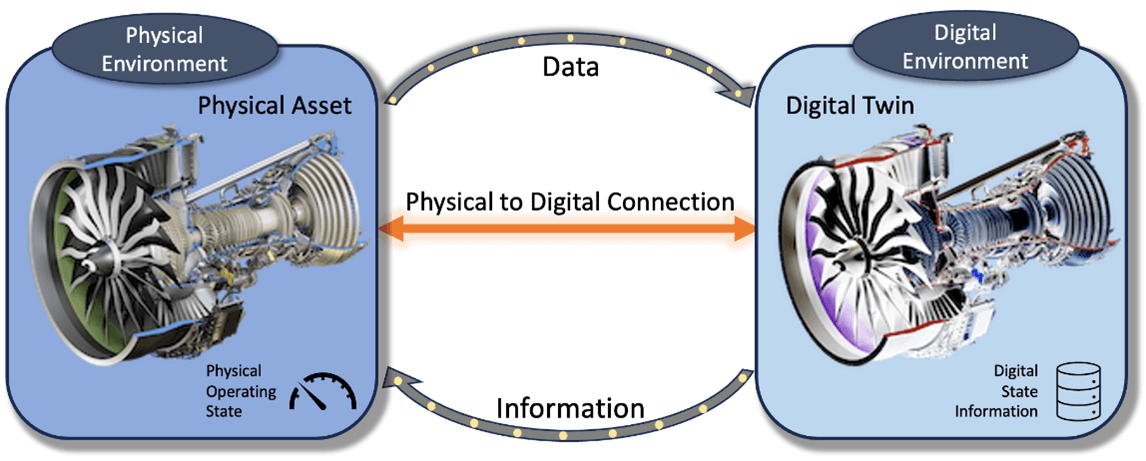
\includegraphics[width=0.8\textwidth]{assets/pics/bab3_1.png}
%     \caption{Ilustrasi hubungan antara physical asset dan digital representation}
%     \label{fig:digital_twin_concept}
% \end{figure}

% Karakteristik utama Digital Twin ada di kemampuan sinkronisasinya secara real-time dengan objek fisik basisnya, kapabilitas analitik prediktif, dan interaktivitas dua arah antara dunia fisik dan digital. Berbeda dengan simulasi tradisional yang umumnya bersifat statis dan dijalankan dalam periode tertentu, Digital Twin beroperasi secara continuous dan terus memperbarui model berdasarkan data terbaru dari sistem fisik (selalu akurat).


% \subsection{Manfaat Digital Twin}

% Digital Twin memberikan berbagai keuntungan signifikan dalam pengelolaan dan optimisasi sistem. Manfaat utama dari implementasi Digital Twin dapat dikategorikan ke dalam beberapa aspek operasional dan strategis.

% \textbf{Simulasi dan Pengujian Tanpa Risiko} memungkinkan simulasi dan testing menyeluruh dari berbagai sistem, konfigurasi, atau skenario tanpa adanya risiko kerugian atau kerusakan sistem akibat perubahan yang tidak sesuai. Kemampuan ini mencakup pemodelan dan analisis performa sistem secara keseluruhan, identifikasi potensi munculnya masalah, dan evaluasi terhadap berbagai konfigurasi yang mungkin untuk mengoptimalkan kinerja tanpa perlu melakukan uji coba fisik yang jauh lebih mahal dan beresiko.

% \textbf{Kemampuan Prediktif dan Maintenance} Digital Twin memiliki fungsi prediktif dengan memungkinkan monitoring dan analisis secara visual dan digital, lengkap dari sistem. Sensor dapat memantau output dari setiap komponen dan menandai masalah yang mungkin terjadi di masa depan untuk memprediksi failure komponen. Hal ini memungkinkan perbaikan dilakukan sebelum masalah terjadi, mengurangi downtime yang tidak terduga, dan menghemat biaya maintenance.

% \textbf{Monitoring Jarak Jauh} Digital Twin memungkinkan monitoring dan pengendalian suatu fasilitas secara remote. Dengan adanya representasi virtual ini, kebutuhan untuk inspeksi langsung dapat dikurangi, terutama dalam lingkungan yang berpotensi berbahaya seperti tambang atau menara tinggi. Hal ini tidak hanya meningkatkan keamanan kerja, tetapi juga mengoptimalkan efisiensi operasional dengan meminimalkan turun tangan manual yang tidak diperlukan.

% \textbf{Optimisasi Performa Real-time} memungkinkan analisis terus-menerus terhadap performa sistem dan penyesuaian parameter operasional secara dinamis. Digital Twin dapat menemukan kemungkinan optimisasi berdasarkan kondisi operasional saat ini dan sebelumnya (historis), serta memberikan rekomendasi untuk meningkatkan efisiensi dan produktivitas sistem.



%-----------------------------------------------------------------------------%
\section{WiFi (Wireless Fidelity)}
%-----------------------------------------------------------------------------%

\subsection{Arsitektur WiFi}

\begin{figure}[htbp]
    \centering
    \includegraphics[width=0.8\textwidth]{assets/pics/bss.png}
    \caption{Ilustrasi arsitektur dasar WiFi}
    \label{fig:wifi_architecture}
\end{figure}

Arsitektur IEEE 802.11 (Wi-Fi) terdiri dari beberapa komponen fundamental yang membentuk jaringan nirkabel \cite{cisco_wifi_6}. Unit dasarnya adalah \textit{Basic Service Set} (BSS), yang terdiri dari sebuah \textit{Access Point} (AP) dan beberapa perangkat klien (\textit{Stations} atau STA). AP berfungsi sebagai jembatan antara perangkat nirkabel dan jaringan kabel. Beberapa BSS dapat digabungkan menjadi sebuah \textit{Extended Service Set} (ESS) menggunakan \textit{Distribution System} (biasanya jaringan Ethernet), yang memungkinkan perangkat untuk berpindah antar-AP secara mulus. Setiap jaringan diidentifikasi oleh \textit{Service Set Identifier} (SSID).

\subsection{Frekuensi dan Channel WiFi}
Wi-Fi umumnya beroperasi pada dua pita frekuensi utama: 2,4 GHz dan 5 GHz. Pita 2,4 GHz menawarkan jangkauan yang lebih luas dan penetrasi sinyal yang lebih baik terhadap halangan seperti dinding, namun memiliki jumlah kanal yang terbatas (hanya 3 kanal yang tidak tumpang tindih) dan rentan terhadap interferensi dari perangkat lain (misalnya, Bluetooth dan microwave). Sebaliknya, pita 5 GHz menyediakan lebih banyak kanal dan kecepatan data yang lebih tinggi, namun dengan jangkauan yang lebih pendek dan penetrasi yang lebih lemah.

\subsection{Metrik Kinerja WiFi}

\begin{figure}[htbp]
    \centering
    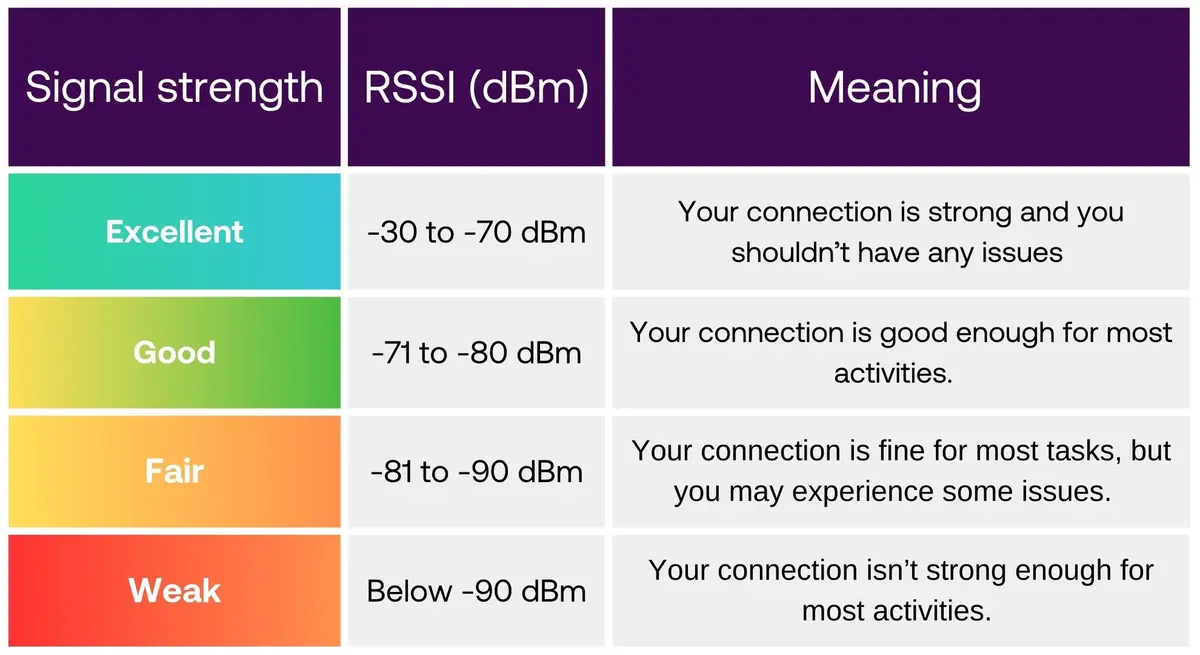
\includegraphics[width=0.8\textwidth]{assets/pics/rssi.png}
    \caption{Tabel kualitas sinyal berdasarkan nilai RSSI}
    \label{fig:rssi}
\end{figure}

Evaluasi kinerja jaringan Wi-Fi dapat dilakukan dengan mengukur berbagai metrik kunci:
\begin{itemize}
    \item \textbf{Received Signal Strength Indicator (RSSI):} Pengukuran kekuatan sinyal yang diterima oleh perangkat, biasanya dinyatakan dalam dBm. Nilai yang lebih tinggi (mendekati 0 dBm) menunjukkan sinyal yang lebih kuat. Sebagai contoh, nilai RSSI di atas -50 dBm dianggap sangat baik, sedangkan di bawah -90 dBm dianggap buruk (Gambar \ref{fig:rssi}).
    \item \textbf{Signal-to-Noise Ratio (SNR):} Rasio antara kekuatan sinyal yang diinginkan dengan tingkat derau (\textit{noise}) di sekitarnya. SNR yang tinggi mengindikasikan kualitas sinyal yang lebih baik.
    \item \textbf{Throughput dan Kapasitas:} Representasi laju data aktual yang dapat dicapai dalam kondisi nyata, yang seringkali lebih rendah dari laju data teoretis karena berbagai faktor seperti \textit{overhead} protokol.
\end{itemize}



%-----------------------------------------------------------------------------%
\section{Jaringan 5G}
%-----------------------------------------------------------------------------%

\subsection{Gambaran Umum Jaringan 5G}
Jaringan 5G adalah standar teknologi seluler generasi kelima yang dirancang untuk memberikan kecepatan data yang jauh lebih tinggi, latensi sangat rendah, dan kapasitas jaringan masif \cite{qualcomm_5g_overview}. Teknologi ini mendukung tiga kategori utama kasus penggunaan: 

\begin{itemize}
    \item \textit{Enhanced Mobile Broadband} (eMBB) untuk aplikasi bandwidth tinggi seperti video 8K dan VR.
    \item \textit{Ultra-Reliable Low-Latency Communications} (URLLC) untuk aplikasi kritis seperti kendaraan otonom dan otomasi industri.
    \item \textit{Massive Machine-Type Communications} (mMTC) untuk menghubungkan miliaran perangkat IoT.
\end{itemize}

\subsection{Arsitektur Jaringan 5G}
Arsitektur 5G mengadopsi \textit{Service-Based Architecture} (SBA), yang berbeda dari arsitektur monolitik generasi sebelumnya. Dalam SBA, fungsi-fungsi jaringan diimplementasikan sebagai layanan mikro (\textit{microservices}) yang berjalan di platform berbasis cloud. Arsitektur ini terdiri dari tiga komponen utama: \textit{User Equipment} (UE) atau perangkat pengguna, \textit{Next-Generation Radio Access Network} (NG-RAN) yang mencakup stasiun pemancar (gNodeB), dan \textit{5G Core} (5GC) yang menjadi pusat kendali jaringan. Desain modular ini memungkinkan fleksibilitas, skalabilitas, dan inovasi yang lebih cepat.

RAN 5G terdiri dari gNodeB yang mengelola komunikasi radio dengan UE. gNodeB dapat dibagi menjadi dua unit: \textit{Centralized Unit} (CU) yang menangani fungsi lapisan atas, dan \textit{Distributed Unit} (DU) yang menangani fungsi lapisan bawah. Pemisahan ini memungkinkan optimisasi sumber daya dan penempatan fungsi jaringan yang lebih efisien.

%-----------------------------------------------------------------------------%
\section{Open Radio Access Network (O-RAN)}
%-----------------------------------------------------------------------------%
Open Radio Access Network (O-RAN) adalah sebuah inisiatif yang bertujuan untuk mentransformasi arsitektur Radio Access Network (RAN) tradisional yang tertutup menjadi ekosistem yang terbuka, cerdas, dan tervirtualisasi \cite{oran_alliance}. Tiga pilar utama O-RAN adalah keterbukaan melalui standardisasi antarmuka untuk interoperabilitas antar vendor, kecerdasan dengan adanya \textit{RAN Intelligent Controller} (RIC) untuk optimisasi berbasis AI/ML, dan virtualisasi fungsi RAN pada perangkat keras komersial.

\subsection{Arsitektur O-RAN}
Arsitektur O-RAN memisahkan (disagregasi) komponen \textit{base station} (gNodeB) menjadi tiga unit utama: \textit{O-RAN Radio Unit} (O-RU) untuk pemrosesan sinyal radio, \textit{O-RAN Distributed Unit} (O-DU) untuk fungsi \textit{real-time} lapisan bawah, dan \textit{O-RAN Centralized Unit} (O-CU) untuk fungsi lapisan atas. Di atas komponen-komponen ini, terdapat sistem manajemen yang terdiri dari \textit{Service Management and Orchestration} (SMO), \textit{Non-Real-Time RAN Intelligent Controller} (Non-RT RIC), dan \textit{Near-Real-Time RAN Intelligent Controller} (Near-RT RIC). Komponen-komponen ini berinteraksi melalui antarmuka terbuka yang terstandarisasi.

\begin{figure}[htbp]
    \centering
    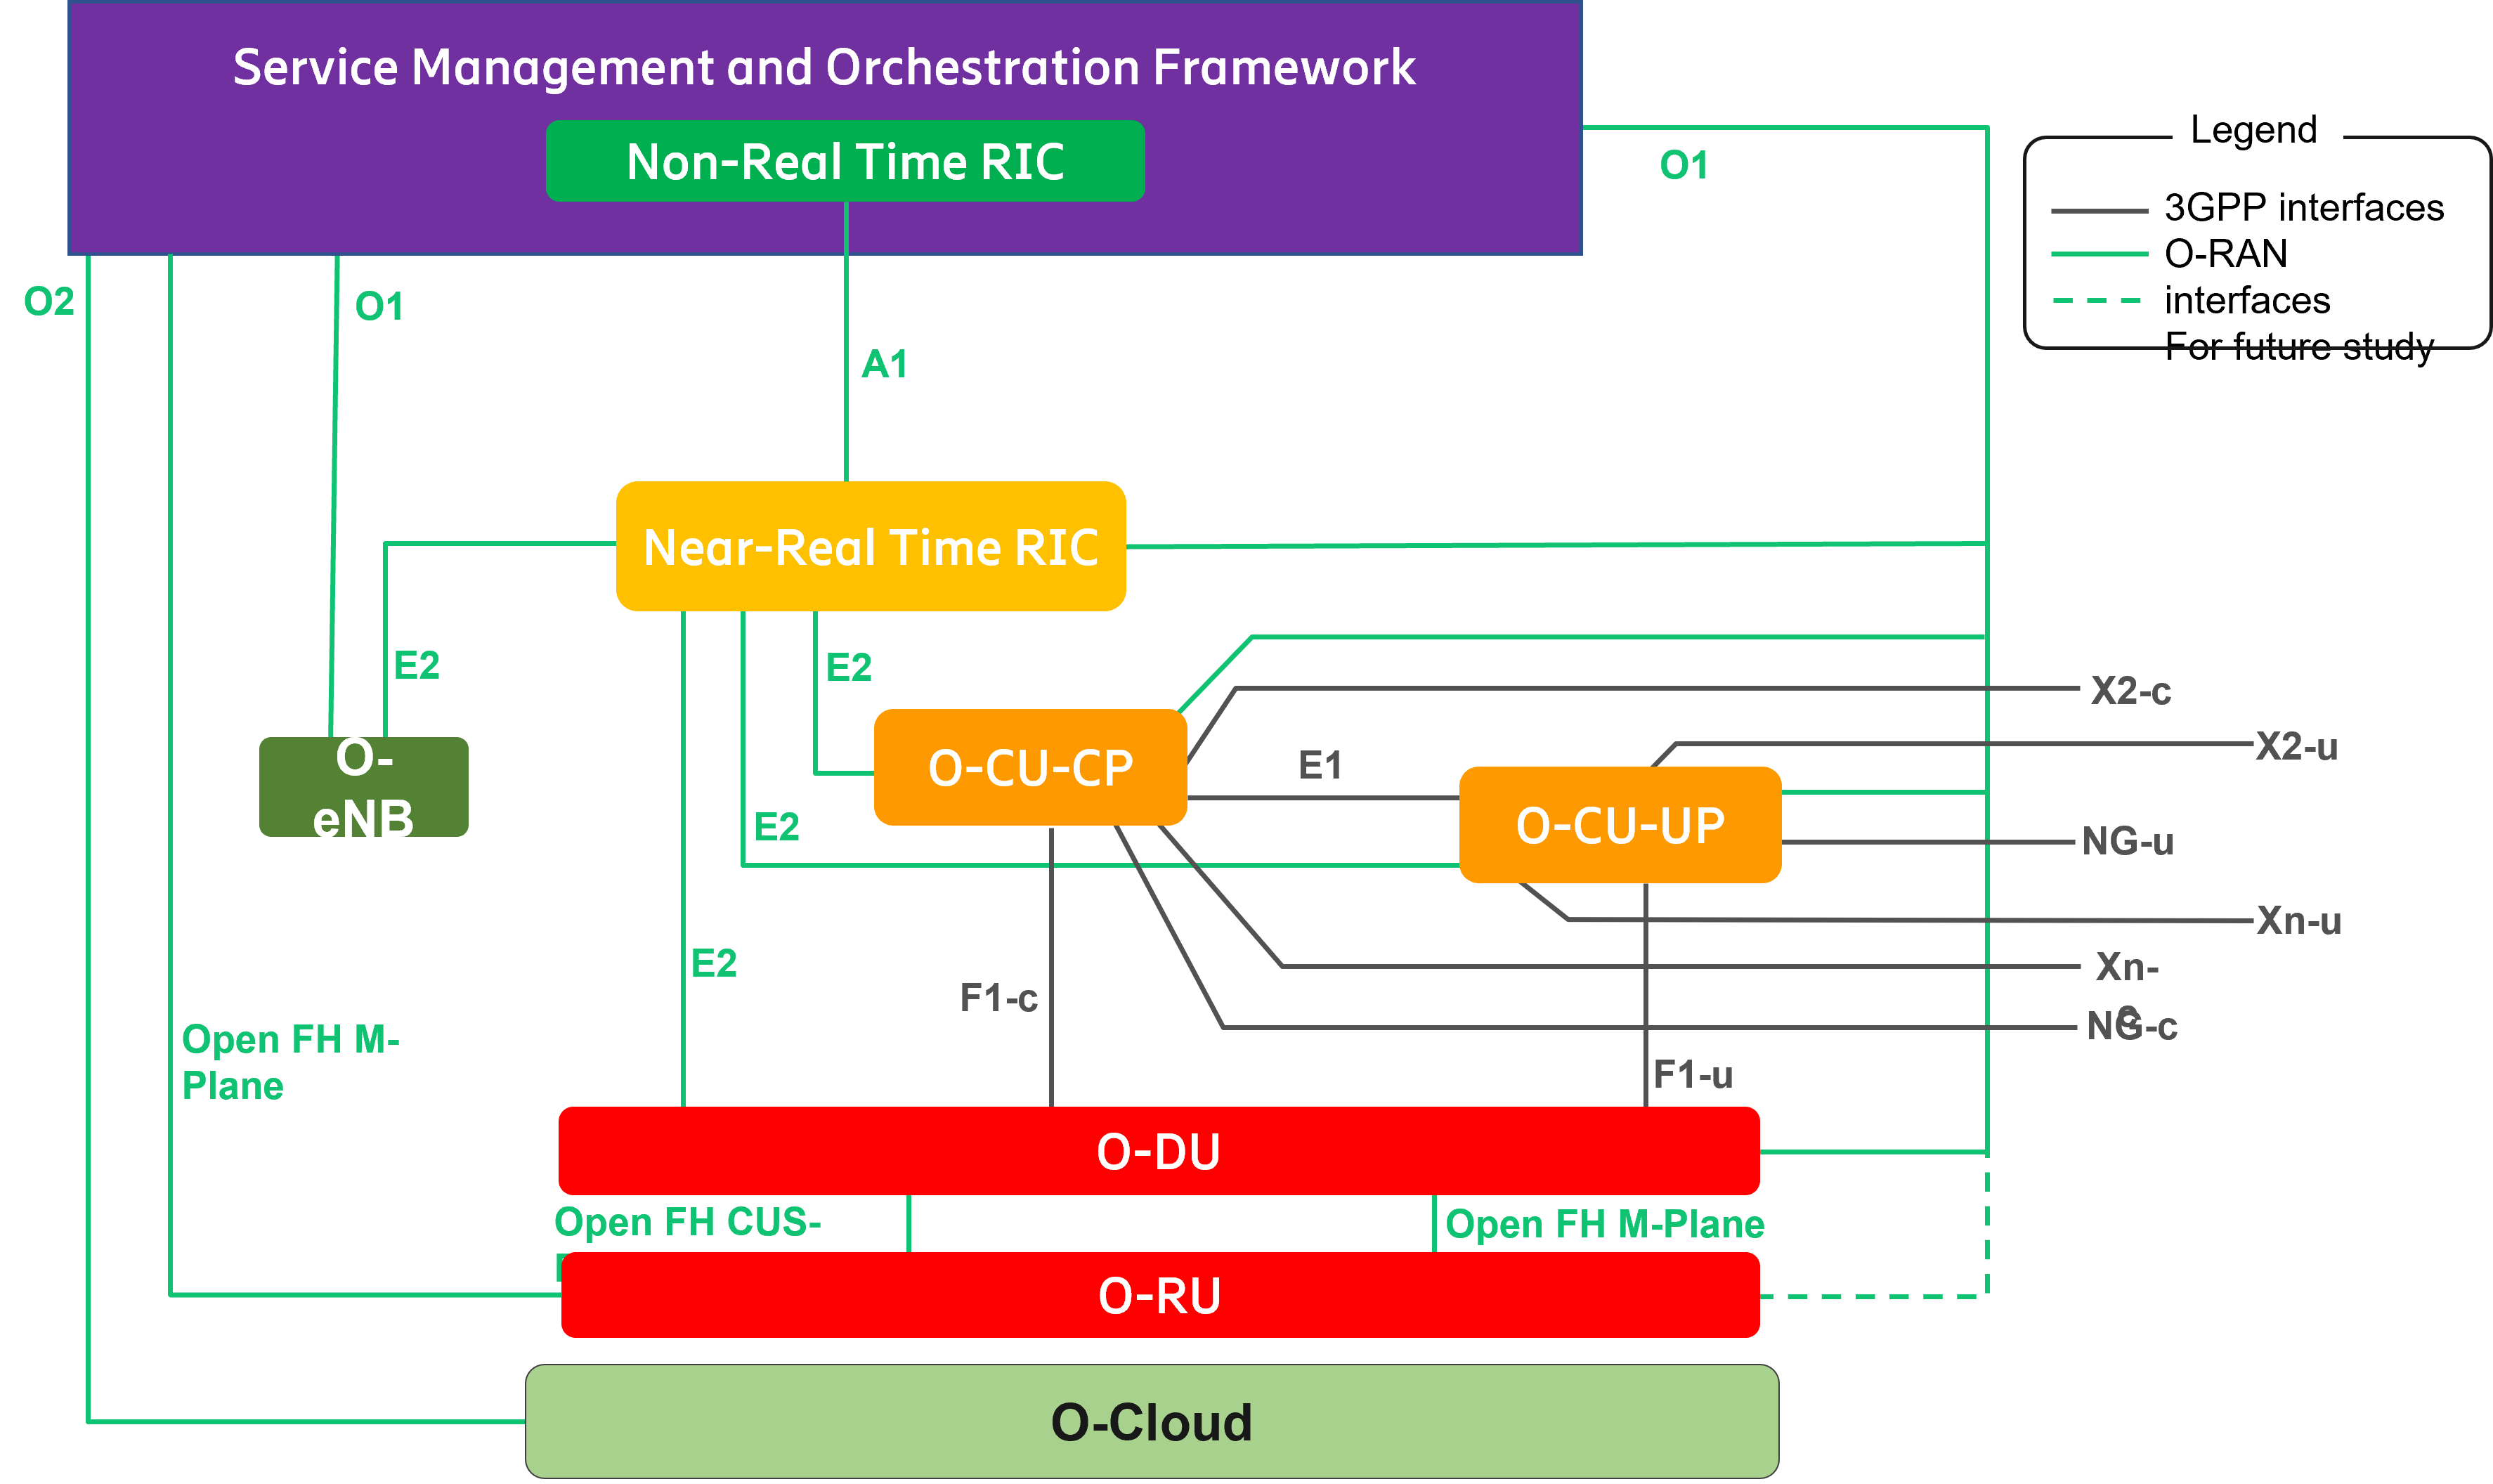
\includegraphics[width=0.8\textwidth]{assets/pics/o-ran-architecture.png}
    \caption{Arsitektur O-RAN}
    \label{fig:oran_architecture}
\end{figure}

\subsection{Service Management and Orchestration (SMO)}
SMO adalah kerangka kerja tingkat tinggi yang bertanggung jawab atas manajemen dan orkestrasi seluruh sumber daya RAN. Dalam konteks integrasi dengan jaringan Wi-Fi, SMO berperan sebagai platform pusat yang mengelola aplikasi (dikenal sebagai rApps) di dalam Non-RT RIC.

SMO berkomunikasi dengan elemen-elemen RAN melalui antarmuka O1 untuk manajemen konfigurasi serta berinteraksi dengan Non-RT RIC melalui antarmuka A1 untuk menetapkan kebijakan dan model AI/ML.

\subsection{Non-Real-Time RIC (Non-RT RIC)}

Non-RT RIC adalah komponen dalam SMO yang menjalankan fungsi fungsi yang tidak memerlukan latensi rendah, biasanya lebih dari satu detik. Fungsi-fungsi yang memerlukan respons cepat ditangani oleh Near-RT RIC. Non-RT RIC menjalankan rApps, yaitu aplikasi yang mengikuti standar dan protokol komunikasi yang ditetapkan O-RAN. Fungsi rApps dapat dirancang untuk menganalisis data performa dari jaringan Wi-Fi dan jaringan seluler untuk membuat keputusan optimisasi.Sebagai contoh, sebuah rApp dapat menganalisis data beban trafik Wi-Fi dan seluler dari waktu ke waktu untuk merekomendasikan perubahan konfigurasi yang dapat meningkatkan efisiensi spektrum atau pengalaman pengguna secara keseluruhan.

\begin{figure}[htbp]
    \centering
    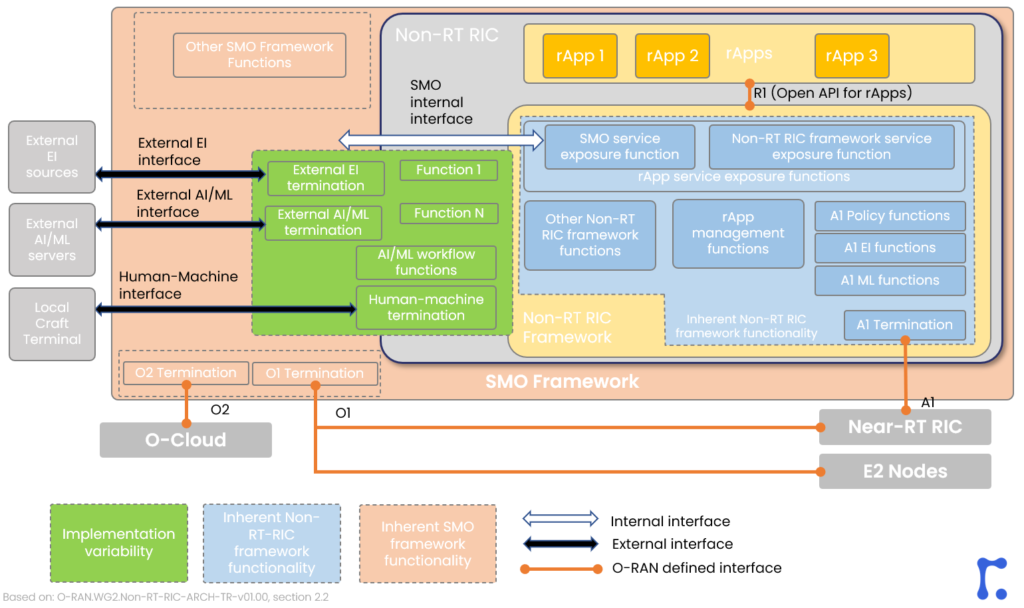
\includegraphics[width=0.8\textwidth]{assets/pics/oran-nonrt.png}
    \caption{Arsitektur Non-RT RIC}
    \label{fig:nonrt_ric_architecture}
\end{figure}

\subsection{Antarmuka O1 dan Virtual Event Streaming (VES)}
Antarmuka O1 adalah saluran manajemen antara SMO dan elemen-elemen jaringan O-RAN (seperti O-CU, O-DU, dan O-RU). Antarmuka ini digunakan untuk tugas-tugas manajemen seperti konfigurasi, pemantauan kinerja, dan penanganan kesalahan (FCAPS). O1 menggunakan protokol NETCONF dengan model data YANG untuk memastikan interoperabilitas.

O-RAN menggunakan mekanisme \textit{streaming} \textit{Virtual Event Streaming} (VES) sehingga SMO harus secara aktif meminta data (polling), elemen jaringan dapat secara proaktif mengirimkan \textit{event} dalam format standar JSON melalui VES Collector. Ini memungkinkan pemantauan  yang lebih efisien dan granular, yang penting untuk mendukung analisis prediktif dan otomasi berbasis \textit{event} di dalam SMO dan Non-RT RIC.

%-----------------------------------------------------------------------------%
\section{NVIDIA Sionna}
%-----------------------------------------------------------------------------%
NVIDIA Sionna adalah sebuah \textit{framework open-source} berbasis TensorFlow yang dirancang untuk simulasi \textit{link-level} dari sistem komunikasi nirkabel \cite{nvidia_sionna}. Keunggulan utamanya adalah kemampuannya untuk melakukan simulasi yang dapat terdiferensiasi (\textit{differentiable}) dan dipercepat oleh GPU. Hal ini memungkinkan integrasi langsung dengan kerangka kerja \textit{machine learning}.

Sionna mampu menghasilkan \textit{Channel Impulse Response} (CIR), yaitu deskripsi lengkap tentang bagaimana sinyal merambat dari pemancar ke penerima melalui berbagai jalur (pantulan, difraksi, dll.). Dari CIR ini, \textit{Received Signal Strength Indicator} (RSSI) dapat dihitung, memberikan gambaran kekuatan sinyal yang diterima.

\begin{figure}[htbp]
    \centering
    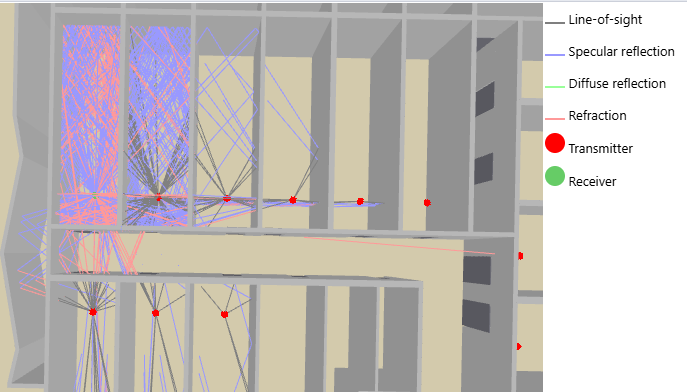
\includegraphics[width=0.8\textwidth]{assets/pics/sionna-simulation.png}
    \caption{Contoh visualisasi simulasi cakupan sinyal menggunakan Sionna}
    \label{fig:sionna_simulation}
\end{figure}

Dalam konteks kerja praktik ini, Sionna digunakan untuk membangun \textit{Digital Twin} dari lingkungan RF dalam ruangan. Dengan memanipulasi berbagai parameter simulasi, performa jaringan dapat dianalisis secara mendalam. Parameter-parameter yang dapat diubah meliputi:
\begin{itemize}
    \item \textbf{Properti Material:} Mengubah nilai permitivitas relatif, konduktivitas, koefisien hamburan (\textit{scattering}), dan ketebalan material seperti beton atau kaca untuk melihat dampaknya pada propagasi sinyal.
    \item \textbf{Konfigurasi Antena:} Menyesuaikan jenis antena (misalnya, \textit{dipole} atau \textit{isotropic}), polarisasi (vertikal, horizontal), dan konfigurasi MIMO.
    \item \textbf{Daya Pancar:} Mengatur daya transmisi dari \textit{access point}.
    \item \textbf{Frekuensi:} Memilih frekuensi operasi, misalnya 2,4 GHz atau 5 GHz.
    \item \textbf{Geometri Lingkungan:} Mengubah tata letak dinding dan objek dalam model 3D.
    \item \textbf{Pengaturan Simulasi:} Mengontrol parameter seperti jumlah pantulan maksimum yang disimulasikan untuk setiap sinar (\textit{ray}).
\end{itemize}
Dengan kemampuan ini, Sionna memungkinkan pembuatan dataset sidik jari (\textit{fingerprint}) RF yang akurat untuk aplikasi lokalisasi dalarssi.webp berbasis AI.